\documentclass[a4paper,12pt]{article}
\usepackage{head}
\usepackage{array}
\usepackage{parskip}

%%%%%%%%%% Global layout %%%%%%%%%%%%%%%%
\usepackage{a4wide,amssymb,epsfig,latexsym,multicol,array,hhline,fancyhdr}
%%%%%%%%%% Encodings %%%%%%%%%%%%%%%%
\usepackage{amsmath} % advanced math extension
\usepackage{comment}
\usepackage{lastpage}
\usepackage[lined,boxed,commentsnumbered]{algorithm2e}
\usepackage{enumerate}
\usepackage{indentfirst}
\usepackage{color}
\usepackage{graphicx} % Standard graphics package
%%%%%%%%%% Better table %%%%%%%%%%%%%%%%
\usepackage{array,booktabs} % customization for table
\usepackage{tabularx, caption}
\usepackage{multirow}
\usepackage{multicol}
%%%%%%%%%%%%%%%%%%%%%%%%%%%%%%%%%%%
\usepackage{rotating} % rotate objects(table,...)
\usepackage{graphics}
\usepackage{geometry} % easier management for page size (margin)
\usepackage{setspace}
\usepackage{epsfig}
%%%%%%%%%%%%%%%%%%%%%%%%%%%%%%%%%%%%%%
\usepackage{hyperref}
\usepackage{pifont}
\usepackage[english]{babel}
\hypersetup{urlcolor=blue,linkcolor=black,citecolor=black,colorlinks=true}
\usepackage{longtable}
\renewcommand{\baselinestretch}{1.5} 


\begin{document}
\pagenumbering{gobble}
\begin{titlepage}
\begin{center}
    \textbf{VIETNAM NATIONAL UNIVERSITY, HO CHI MINH CITY}\\
    \textbf{HO CHI MINH CITY UNIVERSITY OF TECHNOLOGY}\\
    \textbf{Faculty of Computer Science and Engineering}\\

    \vspace{0.5 cm}
    
\includegraphics[scale = 0.3]{Logo.png}\\
    \vspace{0.5 cm}
    \large\textbf{Course:}\\
    \large\textbf{PROBABILITY AND STATISTICS (MT2013)}\\
    \vspace{0.5 cm}
    \begin{tabular}{c}
         \hline\\ \textbf{Project: MEMORY SPEED PREDICTION} \\
         \textbf{BY USING MULTIPLE LINEAR REGRESSION}\\ \\ \hline
    \end{tabular}

\end{center}




\begin{center}
    \begin{tabular}{r l}
        \textbf{Supervisor:}& \textbf{Dr. Nguyen Tien Dung} \\
        Students:&Nguyen Thien Loc - 2252460 \\ 
        &Nguyen Hong Phuc - 2252639 \\ 
        &Ly Trieu Uy  - 2252889 \\ 
        &Le Nhan Van - 2252899 \\ 
        &Che Thanh Vy - 2252937 \\
        Class:&CC01 - Group 25\\
    \end{tabular}
    \\
    \vspace{1 cm}
    \centering\textbf{Ho Chi Minh City, April 2024}
\end{center}
\end{titlepage}


% Start from here

\newpage
\vspace*{0.25 cm}
\textbf{Group contribution:}\\

\begin{longtable}{|c|c|c|}
    \hline
    Members & Contribution & Note\\
    \hline
    Nguyen Thien Loc     & 20\% &\\
    \hline
    Nguyen Hong Phuc     &  20\% & Leader\\
    \hline
    Ly Trieu Uy  &20\% &\\
    \hline
    Le Nhan Van & 20\% &\\ 
    \hline
    Che Thanh Vy & 20\% &\\
    \hline
\end{longtable}

\textbf{Lecturers' assessment:}
\begin{longtable}{|c|p{5 em}|c|}
    \hline
    Members & \centering Grade & Assessment \\
    \hline
    Nguyen Thien Loc     &&   \\
    \hline
    Nguyen Hong Phuc     & &\\
    \hline
    Ly Trieu Uy  && \\
    \hline
    Le Nhan Van & & \\ 
    \hline
    Che Thanh Vy & & \\
    \hline
    
\end{longtable}
\newpage
\pagestyle{fancy}
\pagenumbering{arabic}
\tableofcontents
\vspace*{0.25 cm}
\section{Data Introduction}
\subsection{Dataset descriptions}

The graphics processing unit \textbf{(GPU)} has become one of the most important types of computing technology, both for personal and business computing. Designed for parallel processing, the GPU is used in a wide range of applications, including graphics and video rendering. Although they’re best known for their capabilities in gaming, GPUs are becoming more popular for use in creative production and artificial intelligence (AI).

With the rapid advancement of computer graphics and visualization technologies, GPUs have become essential components in a wide range of applications, including gaming, scientific research, artificial intelligence, and data analysis.

For that reason, this report aims to predict memory speed based on different GPUs by analyzing GPUs' attributes such as Memory\_Speed, Memory, Memory\_Bus, etc., in the dataset.

Data descriptions for the 13 variables are as follows:      



 

\subsection{Variables descriptions}
    \begin{longtable}{|p{11 em}| c|c|p{12 em}|}
        \hline
         Variables & Data type & Unit & Description  \\
         \hline
        Memory\_Speed & Continuous & MHz & Measure of the speed a card can perform texture mapping\\
        \hline
        Memory & Continuous & MB & Dedicated onboard memory used for storing and accessing data needed for graphics processing tasks\\
        \hline
        Memory\_Bus  &  Continuous  &  bit & Type of computer bus, usually in the form of a set of wires or conductor, allow transfers of data and addresses from the main memory to the CPU or a memory controller  \\
        \hline
        Core\_Speed & Continuous & MHz & The speed of the graphics card.\\
        \hline
        Process & Continuous & nm & The size of the smallest features that can be created on the semiconductor chip during manufacturing. \\
        \hline
        Pixel\_Rate &  Continuous & GPixel/s & The number of pixels the graphics processor could write to the video memory \\
        \hline
        Texture\_Rate  & Continuous  & GTexel/s & Measure of the speed with which a particular card can perform texture mapping \\
        \hline
       Memory\_Bandwidth & Continuous &  GB/sec & The amount of information that can be transferred to and from memory per unit time \\
        \hline
        TMUs  & Continuous & None & specialized components responsible for applying textures to 3D objects in graphics rendering\\
        \hline
       Shader  & Continuous & None & a user-defined program designed to run on some stage of a graphics processor \\
        \hline
       Resolution\_WxH & Continuous & None & refers to the width (W) and height (H) dimensions of an image or display, expressed as the number of pixels in each direction \\
        \hline
        Manufacturer & Discrete & None & Manufacturer of the GPU.\\
        \hline
        Memory\_Type  &  Discrete  & None & RAM (Random Access Memory) which can read and write data, and ROM (Read Only Memory) \\
        \hline
    \caption{Variables description} 
    \end{longtable}
\vspace*{.25 cm}

\section{Background}
\subsection{Concept of Multiple linear regression (MLR)}
\tab Multiple linear regression is a statistical method used in various fields to analyze relationships between a dependent variable and two or more independent variables. It extends simple linear regression by incorporating multiple predictors, allowing for a more nuanced understanding of their collective 
influence. The model estimates coefficients for each predictor, indicating their strength and direction of effect. 

\subsection{The model of MLR}
\begin{center}
    $\textbf{y} = \beta_0 + \beta_1 x_1 + \beta_2 x_2 + ... + \beta_n x_n + \epsilon$
\end{center}
\tab where:
\begin{itemize}
    \item $y$ is the dependent variable
    \item $x_i$ is the $i_{th}$ independent variable
    \item $\beta_0$: y-intercept
    \item $\beta_{i}$: coefficient of $x_i$
    \item $\epsilon$: is the error term
\end{itemize}
\subsection{Assumptions of MLR}
\subsubsection{Linearity}
\tab Independent variables and dependent variable shared a linear relationship. 
\subsubsection{Homoscedasticity}

\tab The error term (random disturbance in the 
relationship between the independent variables and the dependent variable) is the same across all values of the independent variables. 

\subsubsection{Independence}
\tab The observations are not influenced by each other. 

\subsubsection{Normality}
\tab The errors are normally distributed. 

\subsection{Advantages of linear regression}
    \begin{itemize}
        \item \textbf{Simplicity and Interpretability:} Linear-regression models are relatively simple and provide an easy-to-interpret mathematical formula that can generate predictions. Linear regression can be applied to various areas in business and academic study.
        \item \textbf{Quick initial insight:} The regression coefficients quickly provide clear insights into the relative importance and effects of each independent variable on the dependent variable even if the relationship is not perfectly linear.
        \item \textbf{Baseline model:} Linear regression is the fundamental model for improving to a more complex model. 
        \item \textbf{Stability:} Particularly in situations when there are few features, linear regression tends to be more stable and less prone to overfitting. Having this can be helpful when working with smaller datasets. 
    \end{itemize}

\subsection{Concept of Random forest regression (RFR)}
\tab Random Forest is a versatile machine learning algorithm that's adept at classification and regression tasks. It constructs a multitude of decision trees during training and combines their predictions to make more accurate and robust predictions compared to individual trees. By leveraging random sampling of data and features, it mitigates overfitting and generalizes well to unseen data. Additionally, it requires minimal hyperparameter tuning, making it easy to use and suitable for a wide range of applications. 

\subsection{Assumptions of RFR}
\subsubsection{Quality of data}
\tab Real values and datasets with no missing value while the input value is continuous and the target variable is discrete are provided for best predictions. 

\subsubsection{Independence of Trees}
\tab Each tree's predictions must have very low correlations.  

\subsubsection{Appropriate Hyperparameters}
\tab While Random Forests are relatively robust to hyperparameters, it is essential to tune them appropriately for optimal performance. Common hyperparameters include the number of trees in the forest, tree depth, minimum samples required for splitting nodes, and the number of features considered for each split. 

\subsection{Advantages of random forest regression}

    \begin{itemize}
        \item \textbf{Quickly applied time:} Random forest regression requires shorter training time than other algorithms.
        \item \textbf{High accuracy:} Predicts output with great accuracy, and it works efficiently even on big datasets and even when significant amount of data is absent.
        \item \textbf{Reduced Bias:} As they combine the predictions of multiple trees, reducing the risk of bias associated with any single tree. 
    \end{itemize}
\section{Descriptive Statistics}
\subsection{Data reading}
\tab We'll use R's read.csv function to import our data. Our focus will be on the following columns: Memory, Resolution, Manufacturer, Core Speed, Memory Bus, Memory Speed, Process, Pixel Rate, Texture Rate, TMUs, Shader, Memory Bandwidth. This emphasis is crucial since our primary goal is to predict Memory Speed.  We'll check each column for missing values, as minimizing these is essential for accurate prediction.:
\begin{center}
    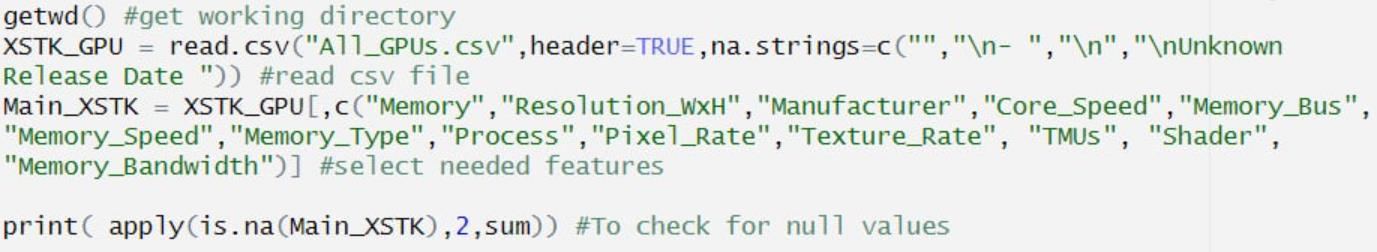
\includegraphics[width=0.8\textwidth]{Read_Data.png}
\end{center}
\tab Then we check for the missing values in the dataset
\begin{center}
    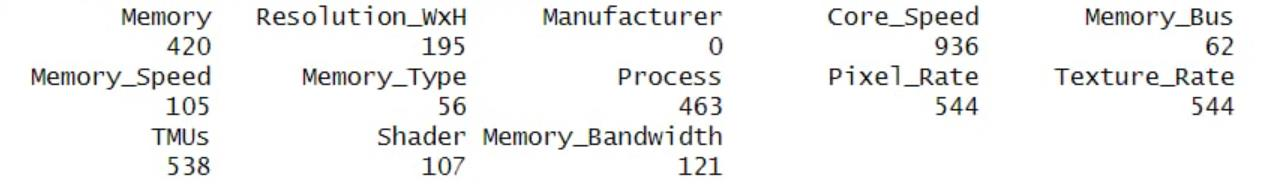
\includegraphics[width=0.8\textwidth]{Checknull.png}
\end{center}
\subsection{Data cleaning}
\tab The missing values comprise less than 30\% of our dataset. Therefore, we'll convert relevant columns to numeric data types and replace N/A values with their corresponding median values to prepare the data for analysis
\begin{center}
    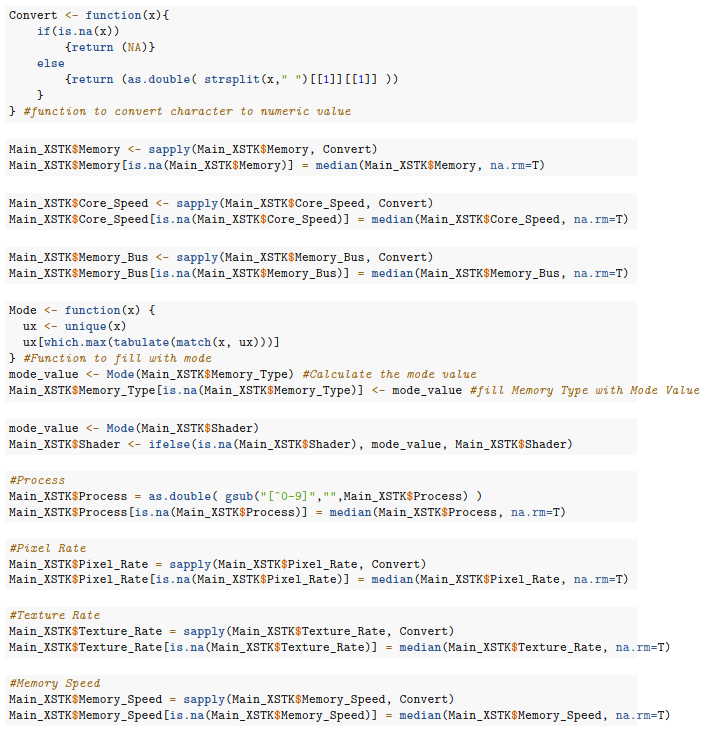
\includegraphics[width=0.8\textwidth]{cleaning.png}
\end{center}

\tab And for some value, we'll use the mode (the most frequent value) to fill in some missing data. This approach helps us preserve the overall shape of the data distribution, especially when dealing with categories
\begin{center}
    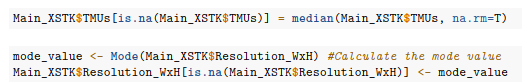
\includegraphics[width=0.8\textwidth]{clean2.png}
\end{center}

\tab After cleaning the data set, we re-check the missing value of the data set again
\begin{center}
    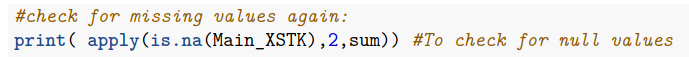
\includegraphics[width=0.8\textwidth]{check.png}
\end{center}
\begin{center}
    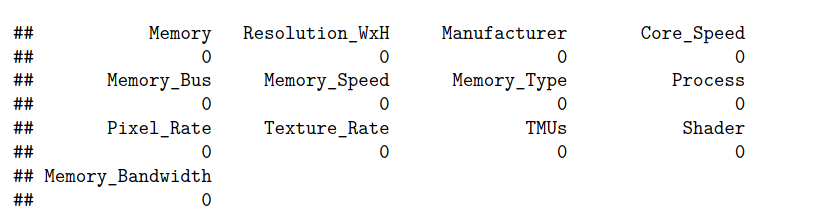
\includegraphics[width=0.8\textwidth]{checked.png}
\end{center}

\tab After checked, There's no missing value in our data set

\subsection{Data visualization}
\subsubsection{Summary table}
\tab We summary all the columns in the data set using "describe"
\begin{center}
    
\includegraphics[width=0.8\textwidth]{des.png}
\end{center}
\begin{center}
    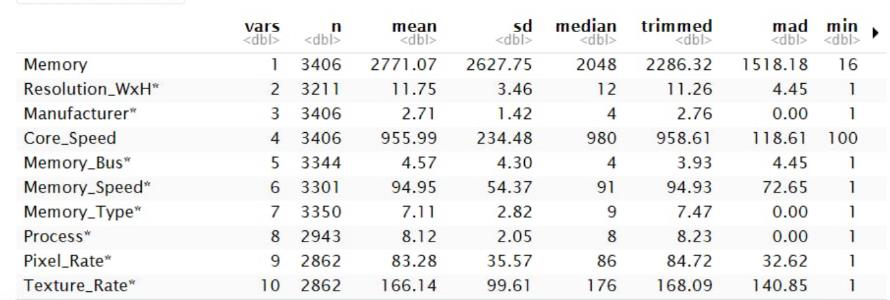
\includegraphics[width=0.8\textwidth]{des1.png}
\end{center}

\subsubsection{Histogram}
\tab Use histograms to analyze the distributions of these 12 key variables: Memory Speed, Memory, Memory Bus, Core Speed, Process, Pixel Rate, Texture Rate, Memory Bandwidth, TMUs, Shader, Resolution WxH, Manufacturer, and Memory Type. This will help us understand their spread, central tendencies, and any potential outliers

\begin{center}
    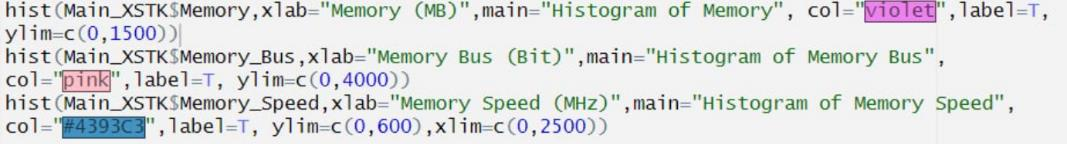
\includegraphics[width=0.7\textwidth]{sk.png}
\end{center}
\begin{center}
    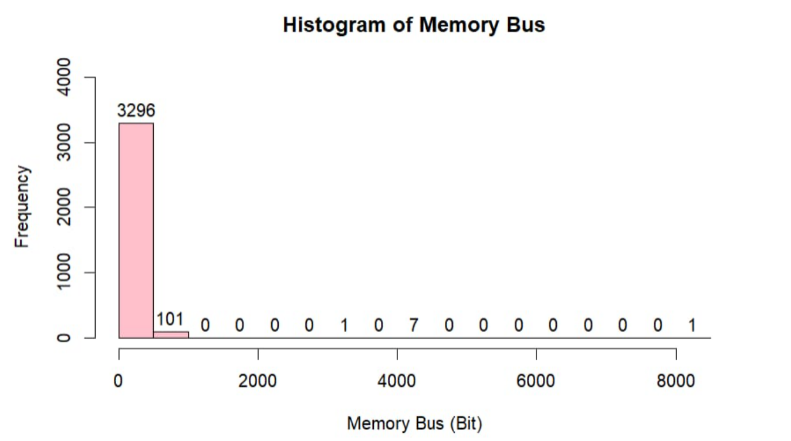
\includegraphics[width=0.7\textwidth]{membush.png}
\end{center}
\begin{center}
    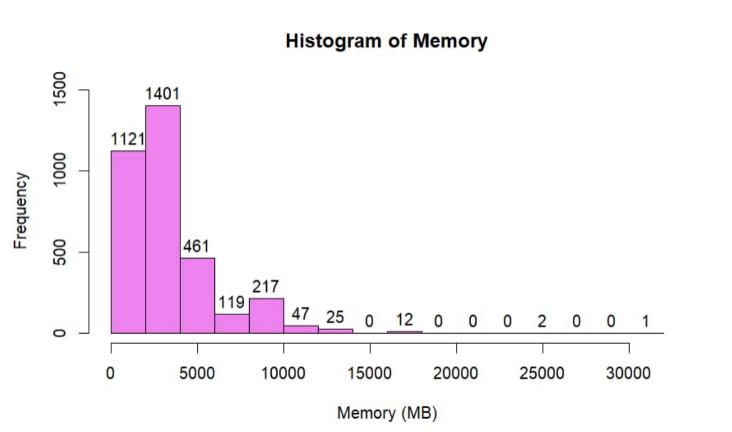
\includegraphics[width=0.7\textwidth]{memh.png}
\end{center}
\begin{center}
    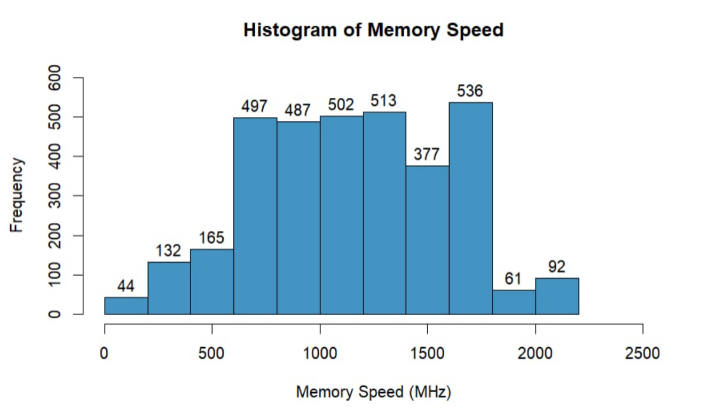
\includegraphics[width=0.7\textwidth]{memspeed.png}
\end{center}

\textbf{Description:}
\begin{itemize}
    \item Histogram of Memory Speed
    \begin{itemize}
        \item The highest frequency is 536 occurs approximately between 1643 and 1786 MHz
        \item The lowest frequency is 44 occurs approximately between 0 and 200 MHz.
        \item This histogram tends to be central.
    \end{itemize}

    \item Histogram of Memory
    \begin{itemize}
        \item The highest frequency is 1401 occurs approximately between 2000 and 4000 MB
        \item The lowest frequency is 0 occurs approximately between 14000 and 16000 MB, from 18000 to 24000 MB, and from 26000 to 30000 MB
        \item This histogram tends to skew left.
    \end{itemize}
    \item Histogram of Memory Bus
    \begin{itemize}
        \item The highest frequency is 3296 occurs approximately between 0 and 5000 Bit.
        \item The lowest frequency is 0 occurs approximately between 1000 and 8000 Bit except from 3000 to 3500 Bit, from 4000 to 4500 Bit and from 8000 to 8500 Bit.
        \item This histogram tends to skew left.
    \end{itemize}
    
\end{itemize}
\textbf{Our next analysis will center on Core Speed, Process, and Pixel Rate.}
\begin{center}
    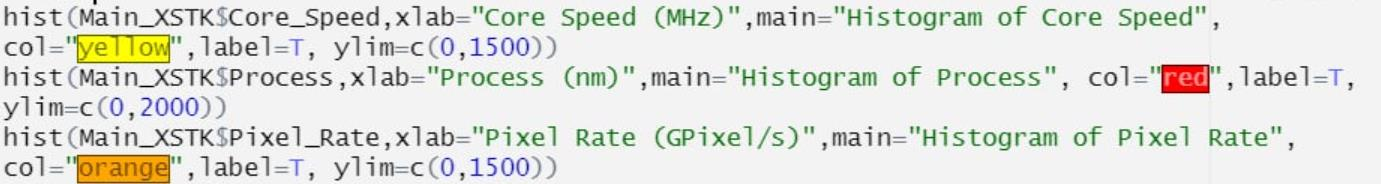
\includegraphics[width=0.7\textwidth]{sk1.png}
\end{center}
\begin{center}
    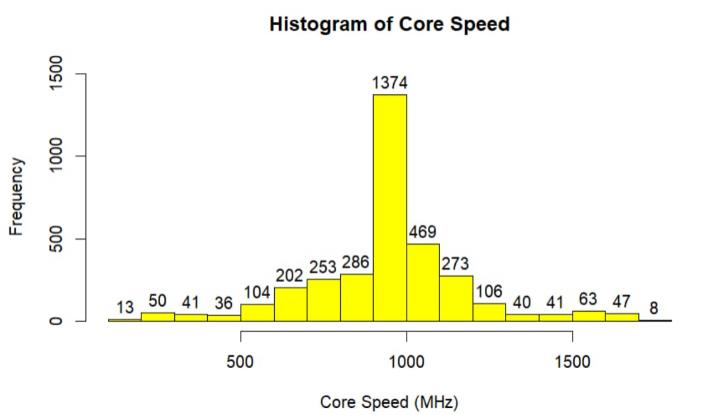
\includegraphics[width=0.7\textwidth]{CSpeed.png}
\end{center}
\begin{center}
    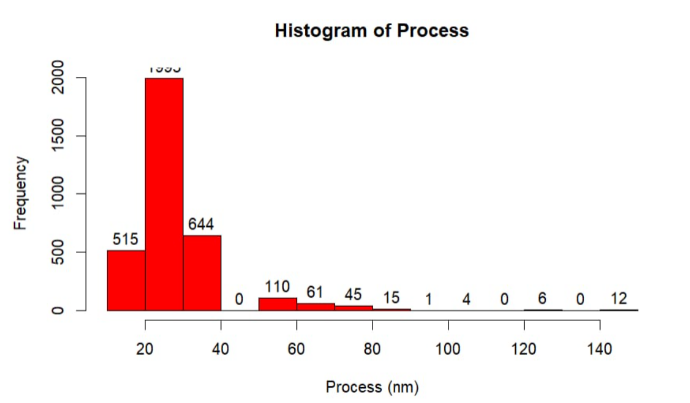
\includegraphics[width=0.7\textwidth]{Process.png}
\end{center}
\begin{center}
    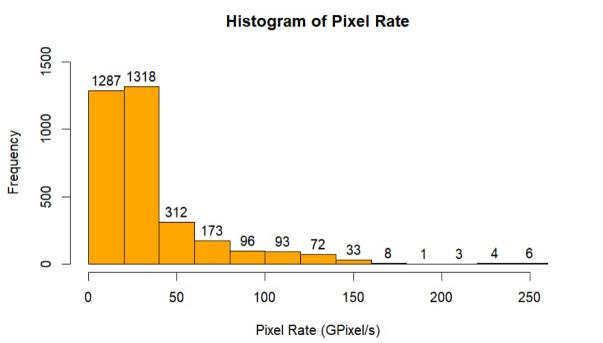
\includegraphics[width=0.7\textwidth]{PixelRatepng.png}
\end{center}

\textbf{Description:}
\begin{itemize}
    \item Histogram of Core Speed
    \begin{itemize}
        \item The highest frequency is 1374 occurs approximately between 900 and 1000 MHz.
        \item The lowest frequency is 8 occurs approximately between 1700 and 1800 MHz.
        \item This histogram tends to be central.
    \end{itemize}

    \item Histogram of Process
    \begin{itemize}
        \item The highest frequency is 1993 occurs approximately between 20 and 30nm.
        \item The lowest frequency is 0 occurs approximately between 40 and 50 MB, from 110 to 120 nm, and from 130 to 140 nm.
        \item This histogram tends to skew left.
    \end{itemize}
    \item Histogram of Pixel Rate
    \begin{itemize}
        \item The highest frequency is 1318 occurs approximately between 20 and 40 GPixel/s.
        \item The lowest frequency is 1 occurs approximately between 180 and 200.
        \item This histogram tends to skew left.
    \end{itemize}
\end{itemize}

\textbf{Now, let's shift our attention to Texture Rate, Memory Bandwith, and TMUs and explore their characteristics.}

\begin{center}
    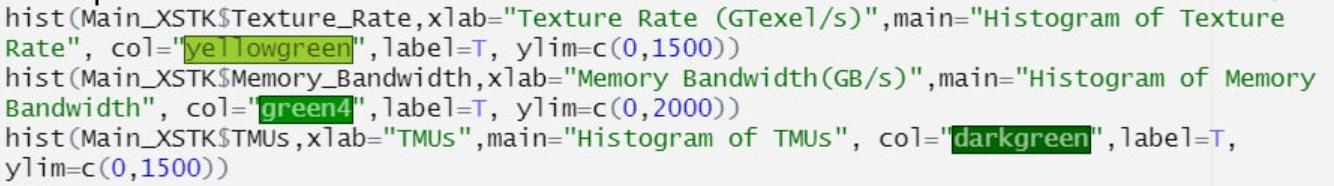
\includegraphics[width=0.7\textwidth]{sk2.png}
\end{center}
\begin{center}
    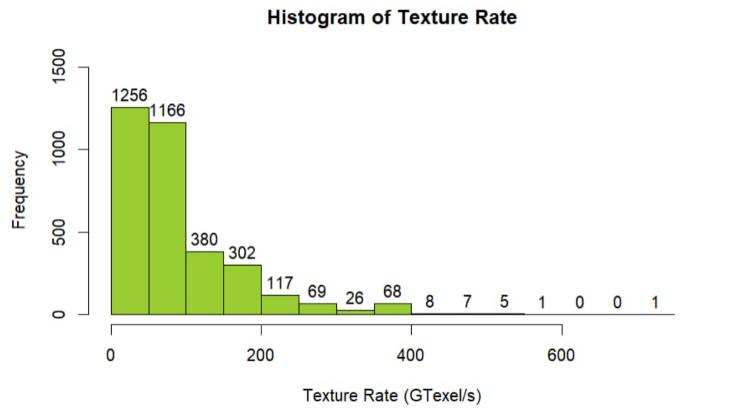
\includegraphics[width=0.7\textwidth]{text.png}
\end{center}
\begin{center}
    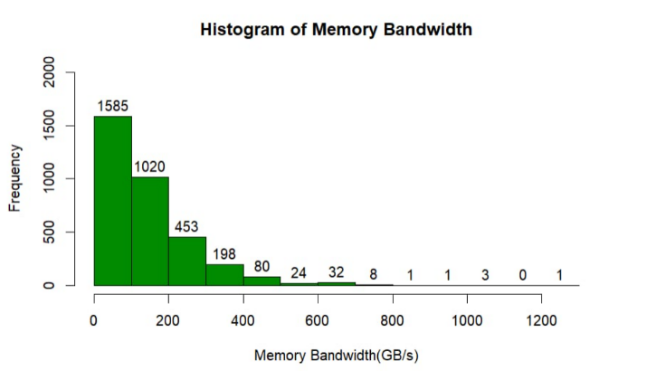
\includegraphics[width=0.7\textwidth]{bandwidth.png}
\end{center}
\begin{center}
    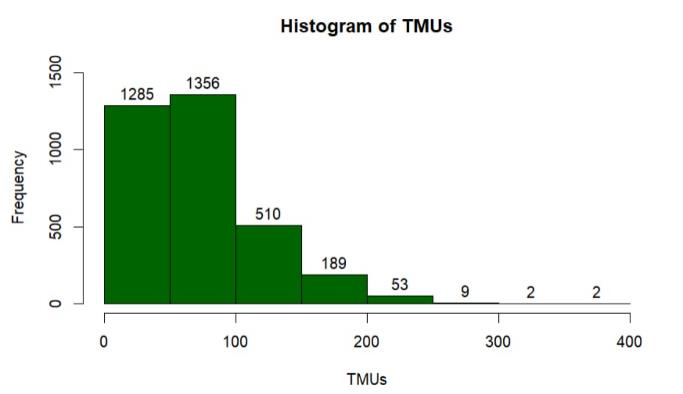
\includegraphics[width=0.7\textwidth]{TMUs.png}
\end{center}


\textbf{Description:}
\begin{itemize}
    \item Histogram of Texture Rate
    \begin{itemize}
        \item The highest frequency is 1256 occurs approximately between 0 and 50 GTexel/s.
        \item The lowest frequency is 0 occurs approximately between 600 and 700 GTexel/s.
        \item This histogram tends to skew left.
    \end{itemize}

    \item Histogram of Memory Bandwidth
    \begin{itemize}
        \item The highest frequency is 1585 occurs approximately between 0 and 100 GB/s.
        \item The lowest frequency is 0 occurs approximately between 1100 and 1200 GB/s.
        \item  This histogram tends to skew left.
    \end{itemize}
    \item Histogram of TMUs
    \begin{itemize}
        \item The highest frequency is 1356 occurs approximately between 50 and 100.
        \item The lowest frequency is 2 occurs approximately between 300 to 400.
        \item This histogram tends to skew left.
    \end{itemize}
\end{itemize}
\textbf{Next, we will analyze Shader, Resolution} 
\begin{center}
    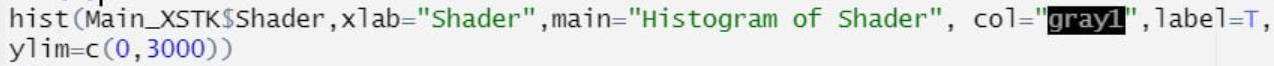
\includegraphics[width=0.7\textwidth]{shader.png}
\end{center}
\begin{center}
    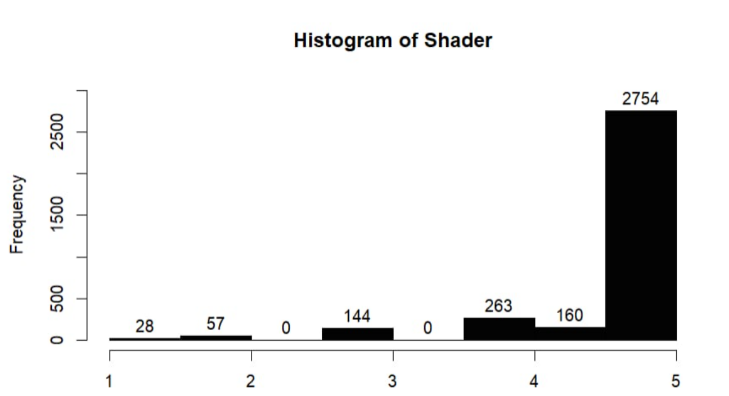
\includegraphics[width=0.7\textwidth]{shader1.png}
\end{center}
\begin{center}
    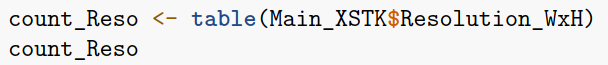
\includegraphics[width=0.7\textwidth]{res.png}
\end{center}
\begin{center}
    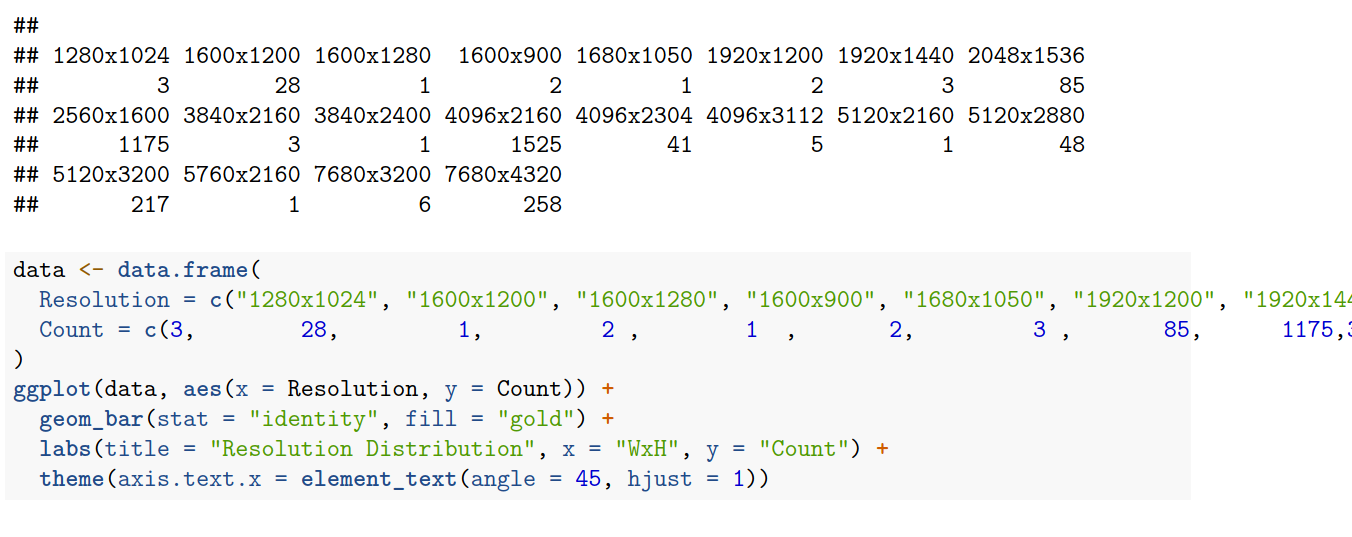
\includegraphics[width=0.7\textwidth]{res1.png}
\end{center}
\begin{center}
    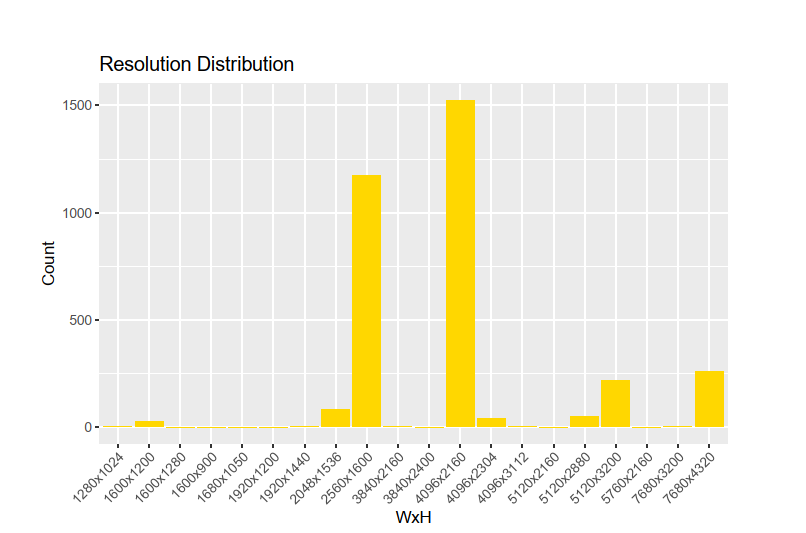
\includegraphics[width=0.7\textwidth]{res2.png}
\end{center}

\textbf{Description:}
\begin{itemize}
    \item Histogram of Shader
    \begin{itemize}
        \item The highest frequency is 2754 occurs approximately between 4.5 and 5.
        \item The lowest frequency is 0 occurs approximately between 2 and 2.5 and from 3 to 3.5.
        \item This histogram tends to skew right.
    \end{itemize}

    \item Histogram of Resolution
    \begin{itemize}
        \item The highest frequency is 1525 occurs at 4096x2160.
        \item The lowest frequency is 1 occurs at 1600x1200, 1600x1280, 1680x1050, 3840x2400, 5120x2160, and 5760x2160.
        \item  This histogram tends to fluctuate.
    \end{itemize}
\end{itemize}

\textbf{Last, we are going to analyze the Memory Type and Manufacturer}

\begin{center}
    
\includegraphics[width=0.7\textwidth]{manu.png}
\end{center}
\begin{center}
    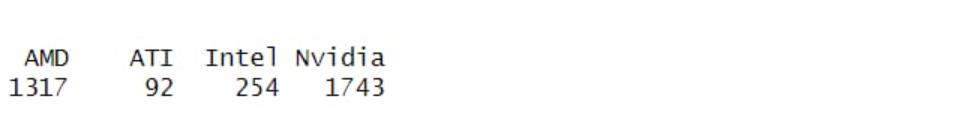
\includegraphics[width=0.7\textwidth]{manu1.png}
\end{center}
\begin{center}
    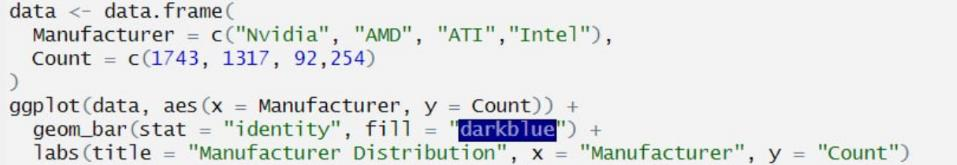
\includegraphics[width=0.7\textwidth]{manu2.png}
\end{center}
\begin{center}
    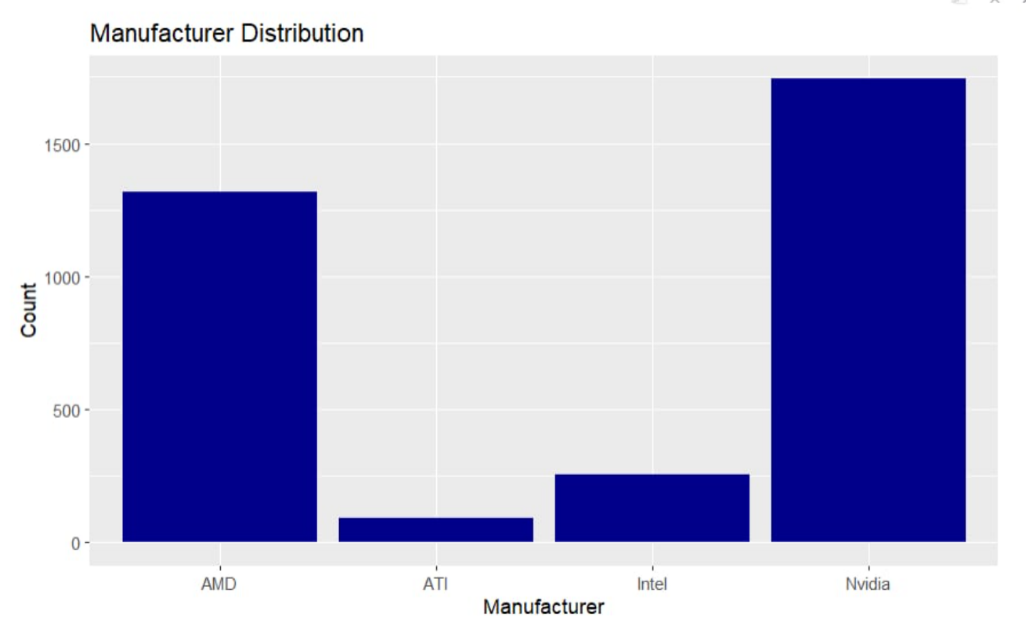
\includegraphics[width=0.7\textwidth]{manu3.png}
\end{center}
\begin{center}
    
\includegraphics[width=0.7\textwidth]{type1.png}
\end{center}
\begin{center}
    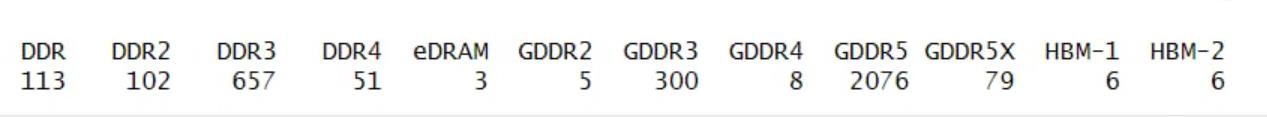
\includegraphics[width=0.7\textwidth]{type2.png}
\end{center}
\begin{center}
    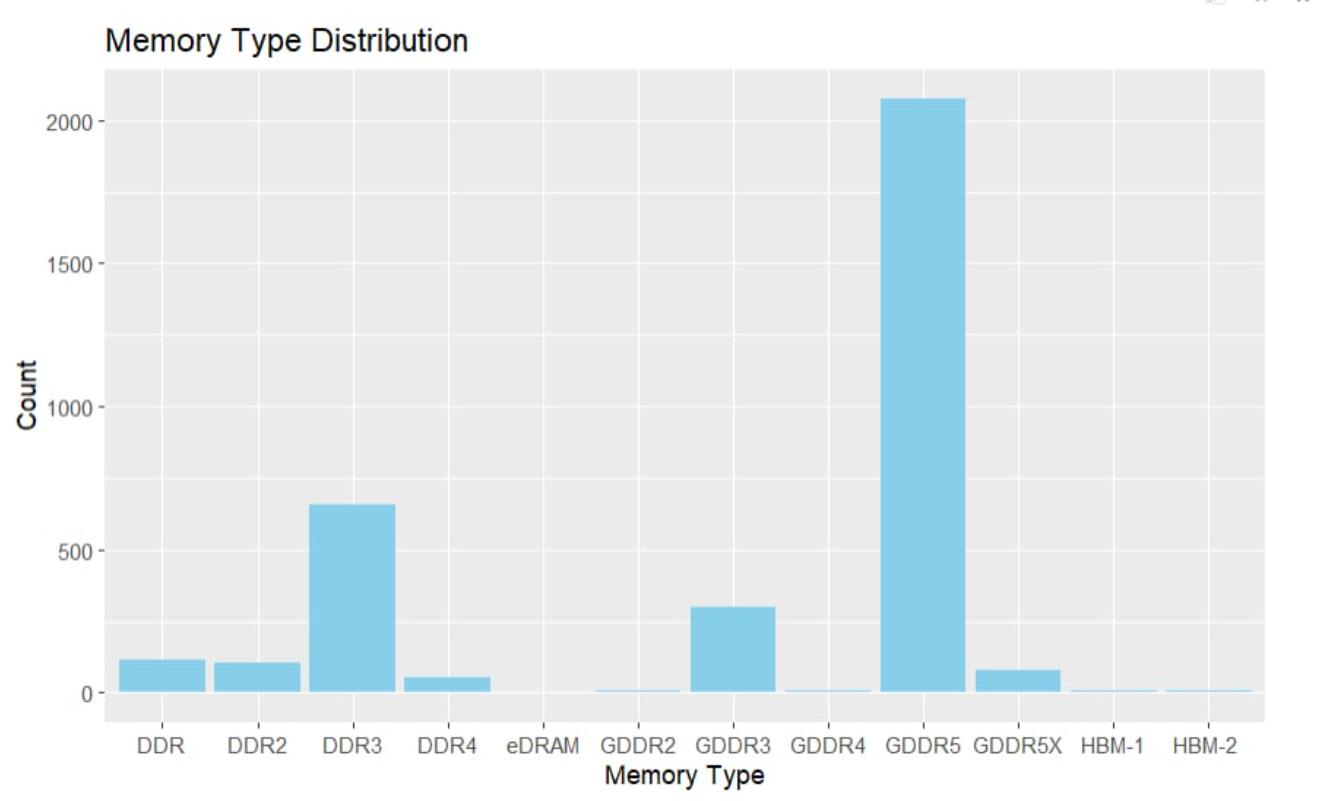
\includegraphics[width=0.7\textwidth]{type3.png}
\end{center}

\textbf{Description:}
\begin{itemize}
    \item Histogram of Memory Type
    \begin{itemize}
        \item The highest frequency is 2754 occurs approximately between 4.5 and 5.
        \item The lowest frequency is 0 occurs approximately between 2 and 2.5 and from 3 to 3.5.
        \item This histogram tends to fluctuate.
    \end{itemize}

    \item Histogram of Manufacturer
    \begin{itemize}
        \item The highest frequency is 1743 occurs at NVIDEA.
        \item The lowest frequency is 92 occurs at ATI., 5120x2160, and 5760x2160.
        \item  This histogram tends to fluctuate.
    \end{itemize}
\end{itemize}

\subsection{Boxplots}
\begin{center}
    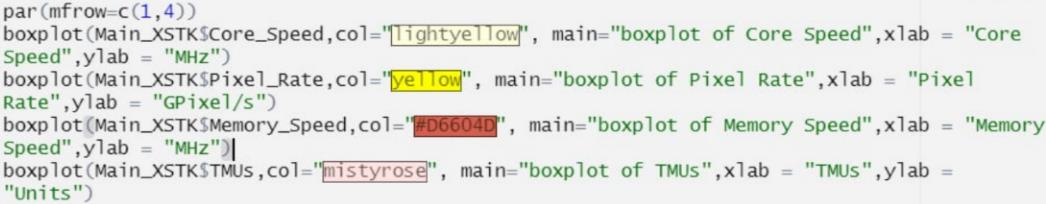
\includegraphics[width=0.7\textwidth]{bp1.png}
\end{center}
\begin{center}
    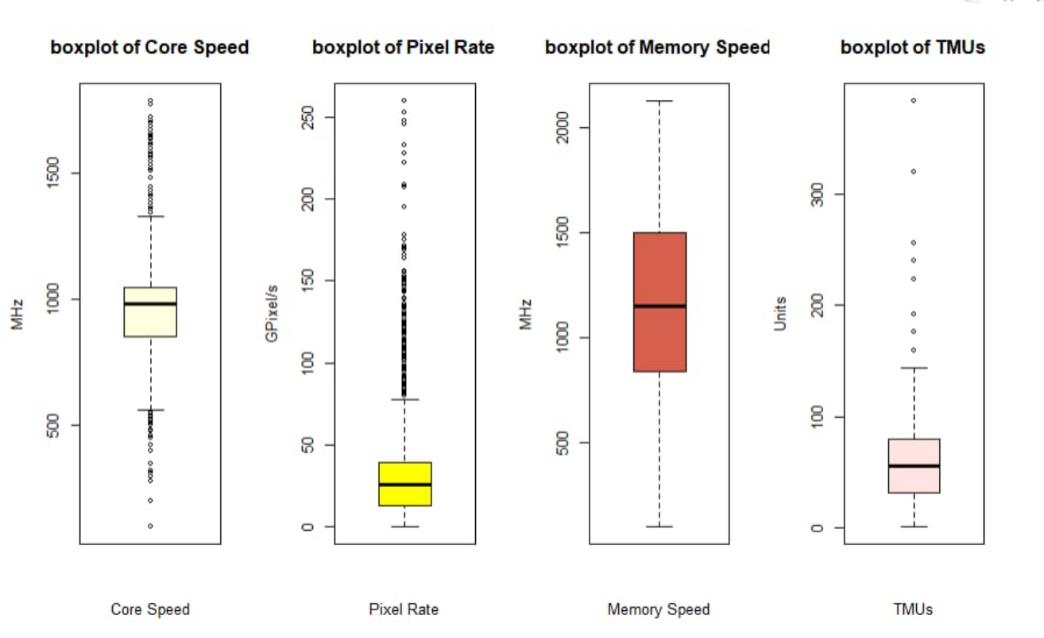
\includegraphics[width=0.7\textwidth]{bp2.png}
\end{center}
\begin{center}
    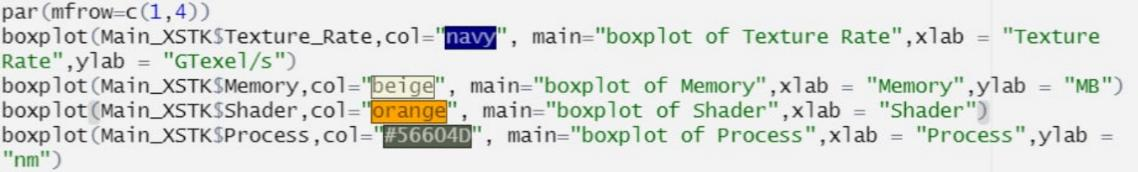
\includegraphics[width=0.7\textwidth]{bp3.png}
\end{center}
\begin{center}
    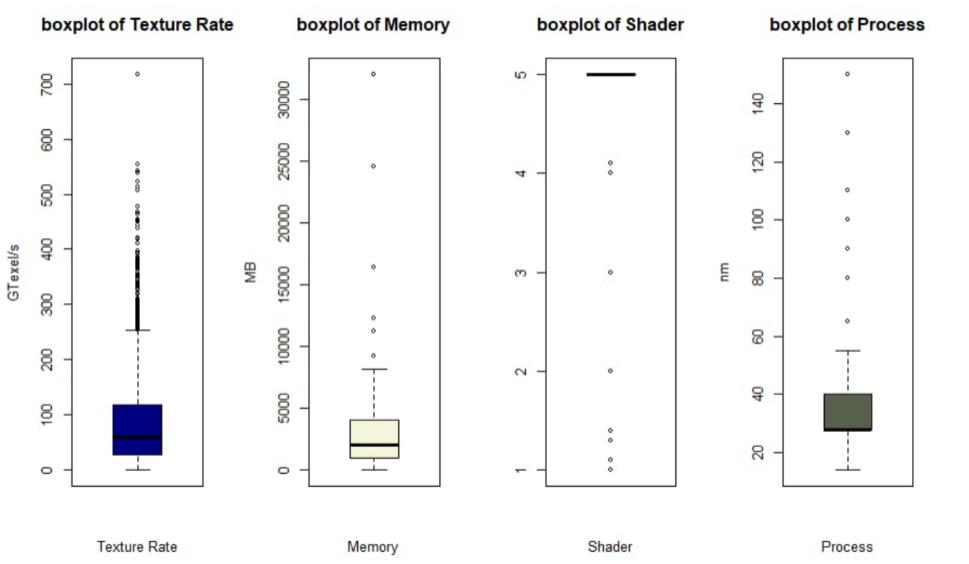
\includegraphics[width=0.7\textwidth]{bp4.png}
\end{center}
\begin{center}
    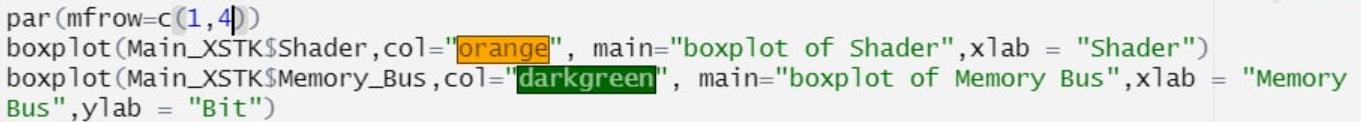
\includegraphics[width=0.7\textwidth]{bp5.png}
\end{center}
\begin{center}
    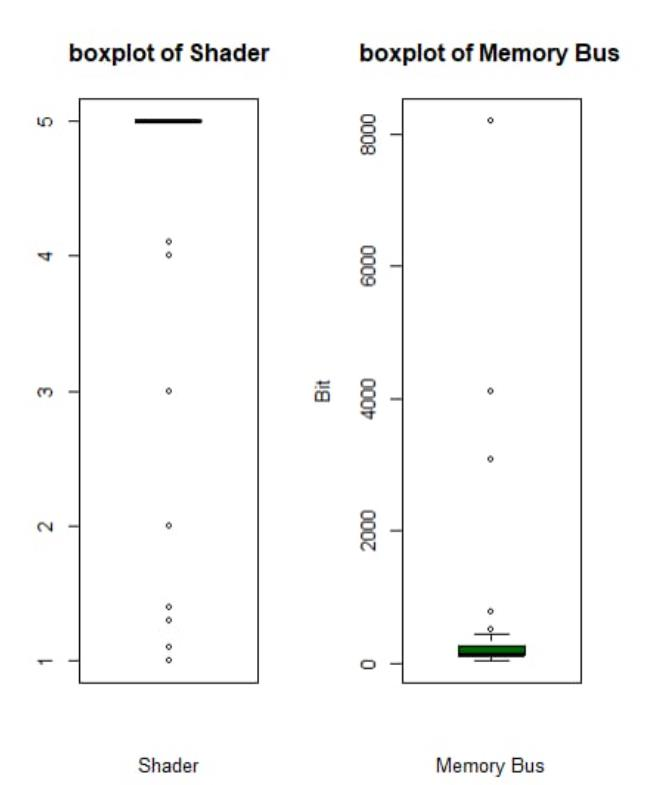
\includegraphics[width=0.7\textwidth]{bp6.png}
\end{center}
\tab \textbf{Comment:} We observe that each output is based on input data that is distributed and exhibits in a similar pattern except for Memory Speed with a wider value range and Shader with tiny range of value. It is not feasible to accurately predict the price by solely considering one variable
\section{Inferential Statistic}
\tab We plan to construct a Multiple Linear Regression (MLR) model where Memory\_Speed serves as the output or dependent variable. The independent variables, including Memory, Memory\_Bandwidth, Core\_Speed, Memory\_Bus, Memory\_Type, Process, Texture\_Rate, and Pixel\_Rate, will be utilized. Our aim is to predict the missing values of Memory\_Speed in the original dataset using the MLR model, while also examining the relationship between Memory\_Speed and the independent variables. Following the assessment of MLR assumptions, aside from normality, we proceed with splitting the dataset and constructing the model.

\subsection{Sample splitting}
\tab We partitioned the dataset into training and testing subsets to ensure accurate model evaluation. Initially, the model is trained using the training data, followed by refinement using the test data. It's essential to note that evaluating the model solely on the training data is insufficient as it may not generalize well to unseen data.  

\tab For this project, we opted for an 80/20 ratio of training to testing data. 

\begin{center}
    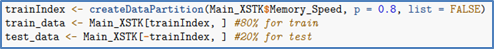
\includegraphics[width=0.8\textwidth]{Sample-splitting.png}
\end{center}

\subsection{Importance of variables}
\tab Higher the value of mean decrease accuracy or mean decrease gini score, higher the importance of the variable in the model. In the plot shown above, Memory\_Bandwidth is most important variable. 

\begin{center}
    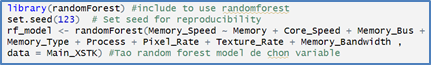
\includegraphics[width=0.8\textwidth]{importance.png}
\end{center}

\begin{center}
    
\includegraphics[width=0.8\textwidth]{importance1.png}
\end{center}

\begin{center}
    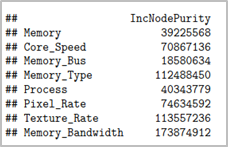
\includegraphics[width=0.7\textwidth]{importance2.png}
\end{center}

\begin{center}
    
\includegraphics[width=0.4\textwidth]{importance3.png}
\end{center}

\begin{center}
    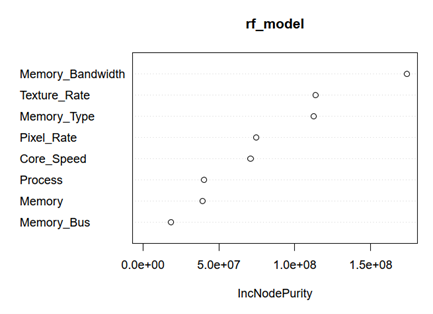
\includegraphics[width=0.8\textwidth]{importance4.png}
\end{center}

\subsection{Building multiple linear regression model}

\begin{center}
    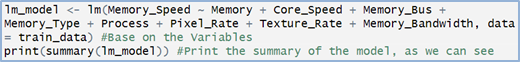
\includegraphics[width=0.8\textwidth]{Build-model.png}
\end{center}

\begin{center}
    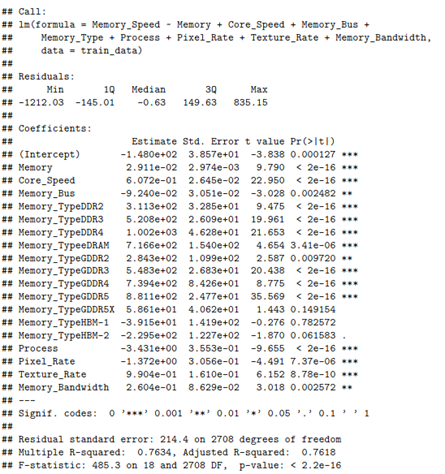
\includegraphics[width=0.8\textwidth]{Build-model1.png}
\end{center}

\tab The variables Memory\_TypeGDDR5X, Memory\_TypeHBM-1, and 
Memory\_TypeHBM-2 are not statistically significant as their p-values are much greater than 0.05. This indicates that these variables do not make a significant contribution to the model and can be removed. Residual standard error stands at 214.4, indicating that actual GPU prices may deviate from the true regression line by roughly 214.4 USD. 

\tab Adjusted R-squared value of 0.7634 indicates that approximately 76.34\% of the variability in the data can be explained by the model. In this case, with an F-statistic of 485.3 and a p-value below 0.05, we can confidently reject the null hypothesis. This means that there is strong evidence to suggest that at least one of the independent variables included in the model is related to the dependent variable (Memory\_Speed). Therefore, we have reason to believe that there is a relationship between the independent variables and the dependent variable.

\subsection{Test for assumptions}
\subsubsection{Assumption 1: Linearity of the Data}
\tab We can check the linearity of the data by looking at the Residual versus Fitted plot. 

\begin{center}
    
\includegraphics[width=0.4\textwidth]{test-ass1.1.png}
\end{center}

\begin{center}
    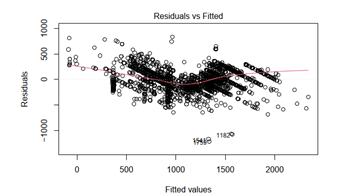
\includegraphics[width=0.8\textwidth]{test-ass1.2.png}
\end{center}
\tab  This red line is not too straight on the 0 line, but it's still acceptable for this model.

\subsubsection{Assumption 2: Predictors (x) are Independent \& Observed with Negligible Error}

\tab The easiest way to check the assumption of independence is using the Durbin-Watson test. 

\begin{center}
    
\includegraphics[width=0.4\textwidth]{test-ass2.1.png}
\end{center}

\begin{center}
    \includegraphics[width=0.8\textwidth]{test-ass2.2.png}
\end{center}

\tab The null hypothesis states that the errors are not auto-correlated with themselves (they are independent). Thus, if we achieve a $p-value >$ 0.05, we would fail to reject the null hypothesis. This would give us enough evidence to state that our independence assumption is met!

\subsubsection{Assumption 3: Residual Errors have a Mean Value of Zero}

\begin{center}
    \includegraphics[width=0.8\textwidth]{test-ass3.1.png}
\end{center}

\begin{center}
    \includegraphics[width=0.8\textwidth]{test-ass3.2.png}
\end{center}

\tab  This value is $-2.14\cdot 10^{-14}$, approximate 0, so this assumption has been met. 

\subsubsection{Assumption 4: Residual Errors have Constant Variance}

\begin{center}
    \includegraphics[width=0.4\textwidth]{test-ass4.1.png}
\end{center}

\begin{center}
    \includegraphics[width=0.8\textwidth]{test-ass4.2.png}
\end{center}

\tab Ideally, we would want to see the residual points equally spread around the red line, which would indicate constant variance. However, it is acceptable. 

\subsubsection{Assumption 5: Testing for normality of the errors}

\tab To check this, we have to use $Q-Q$ plot for normality consideration. The output we expect that the residuals will mostly scatter close to the straight line to get normality hypothesis accepted. 

\begin{center}
    \includegraphics[width=0.4\textwidth]{test-ass5.1.png}
\end{center}

\begin{center}
    \includegraphics[width=0.8\textwidth]{test-ass5.2.png}
\end{center}

\tab We can conclude that this model can be normally accurate, not 100\% accurate. Perhaps another model will be more fitted for this data. 

\subsubsection{Testing for accuracy}

\begin{center}
    \includegraphics[width=0.8\textwidth]{test-accuracy1.png}
\end{center}

\tab In an ideal scenario, where the predicted memory speeds perfectly match the actual memory speeds, all the points would fall on a diagonal line with a slope of 1 (y = x). Deviations from this diagonal line indicate discrepancies between the actual and predicted values.  

\begin{center}
    \includegraphics[width=0.8\textwidth]{test-accuracy2.png}
\end{center}

\begin{center}
    \includegraphics[width=0.8\textwidth]{test-accuracy3.png}
\end{center}

\begin{center}
    \includegraphics[width=0.8\textwidth]{test-accuracy4.png}
\end{center}

\tab  By examining the histogram of residuals, you can assess 
whether the residuals are approximately normally distributed, 
which is an assumption of many linear regression models. If the histogram shows a roughly bell-shaped curve, it suggests that the assumption is reasonable.  

\begin{center}
    \includegraphics[width=0.8\textwidth]{test-accuracy5.png}
\end{center}

\begin{center}
    \includegraphics[width=0.8\textwidth]{test-accuracy6.png}
\end{center}

\begin{center}
    \includegraphics[width=0.8\textwidth]{test-accuracy7.png}
\end{center}

\tab This dataset is ranged from 10 to ~1700 so this error can be assume as small value so it can be accepted. 

\begin{center}
    \includegraphics[width=0.5\textwidth]{test-accuracy8.png}
\end{center}

\begin{center}
    \includegraphics[width=0.5\textwidth]{test-accuracy9.png}
\end{center}

\subsection{Building random forest model}

\begin{center}
    \includegraphics[width=0.3\textwidth]{build-forest1.png}
\end{center}

\begin{center}
    \includegraphics[width=0.8\textwidth]{build-forest2.png}
\end{center}

\tab where:
\begin{itemize}
    \item \textbf{Type of Random Forest:} Indicates whether the Random Forest model is used for regression or classification. In this case, it is a regression Random Forest, meaning it is used for predicting numeric values (Memory\_Speed). 
    \item \textbf{Number of Trees:} Specifies the number of decision trees created by the Random Forest algorithm. Random Forest builds multiple decision trees and combines their predictions to improve the accuracy and robustness of the model. In this example, the model consists of 500 decision trees.
    \item \textbf{No. of Variables Tried at Each Split:} Indicates the number of predictor variables considered for each split in the decision trees. Random Forest randomly selects a subset of predictor variables at each split to create diverse trees. In this example, 4 predictor variables are tried at each split.
    \item \textbf{Mean of Squared Residuals:} The mean of the squared differences between the actual values and the predicted values (residuals) of the target variable (Memory\_Speed). It provides a measure of the model's accuracy. A lower value indicates better performance, as it means the model's predictions are closer to the actual values. (5810.36 is a really good outcome, better than linear regression(x2)). 
    \item \textbf{\%Var:} The percentage of variance explained by the mode, the higher the \%Var, the better the model.
    
\end{itemize}

\begin{center}
    \includegraphics[width=0.4\textwidth]{build-forest3.png}
\end{center}

\begin{center}
    \includegraphics[width=0.8\textwidth]{build-forest4.png}
\end{center}

\subsubsection{Test for accuracy}

\begin{center}
    \includegraphics[width=0.8\textwidth]{test-forest1.png}
\end{center}

\begin{center}
    \includegraphics[width=0.8\textwidth]{test-forest2.png}
\end{center}

\begin{center}
    \includegraphics[width=0.8\textwidth]{test-forest3.png}
\end{center}

\begin{center}
    \includegraphics[width=0.8\textwidth]{test-forest4.png}
\end{center}

\begin{center}
    \includegraphics[width=0.8\textwidth]{test-forest5.png}
\end{center}

\begin{center}
    \includegraphics[width=0.8\textwidth]{test-forest6.png}
\end{center}

\begin{center}
    \includegraphics[width=0.8\textwidth]{test-forest7.png}
\end{center}

\tab $\rightarrow$ This Value is really near 1, so this may be the most fit model for our dataset.

\begin{center}
    \includegraphics[width=0.8\textwidth]{test-forest8.png}
\end{center}

\begin{center}
    \includegraphics[width=0.8\textwidth]{test-forest9.png}
\end{center}

\begin{center}
    \includegraphics[width=0.8\textwidth]{test-forest10.png}
\end{center}

\tab $\rightarrow$ The ideally output is the distribution perfectly lines on the $x – axis$. Therefore, this output is acceptable. 

\begin{center}
    \includegraphics[width=0.6\textwidth]{test-forest11.png}
\end{center}

\begin{center}
    \includegraphics[width=0.5\textwidth]{test-forest12.png}
\end{center}
\section{Discussion and Extension}
\tab The normality assumption is a core requirement in traditional linear regression, which assumes that the residuals adhere to a normal distribution. However, our multiple linear regression (MLR) model does not meet  this assumption (Histogram of Residuals does not meet the normality assumption), raising doubts about the validity of certain inference techniques. Below, we explore the consequences and possible causes of this deviation from normality in residuals. 
\begin{itemize}
        \item \textbf{Outliers:} The presence of outliers, which are data points that significantly deviate from the rest of the dataset, can strongly affect the normality of residuals. These outliers may skew the distribution of residuals and lead to violations of the normality assumption in statistical analyses. 
        \item \textbf{Reliability of Inference:} all Violating the normality assumption can impact the reliability of statistical inferences, such as confidence intervals and hypothesis tests for regression coefficients. 
        \item \textbf{Prediction Interval:} While point predictions of the model may remain valid, prediction intervals could be affected, inaccurately reflecting the uncertainty of individual predictions. 
        \item \textbf{Robustness in Larger Samples:} In larger samples, the Central Limit Theorem may mitigate the impact of non-normality, but caution is still necessary, particularly in smaller samples. 
        \item \textbf{Potential Causes of Non-Normality:} Model misspecification or the presence of outliers may lead to non-normal residuals.
        \item \textbf{Data preprocessing:} Filling a large number of cells with the same repetitive value can introduce several types of errors during data preprocessing and analysis. 
        
    \end{itemize}
\section{Data and code availability}
Data source: \href{https://www.kaggle.com/datasets/iliassekkaf/computerparts?resource=downlo}{data}
\\
Code source: \href{https://drive.google.com/drive/folders/1GeL4okZ9_bs0lAlA93FajCUkQ8V4jnou?usp=sharing&fbclid=IwZXh0bgNhZW0CMTAAAR1_dfD-snUrBtV4fBlCqpO4f8hrxA5yU9OEiGS65ExcUMwF-cCHH7x44LA_aem_AYiTgyF-0HZhQORg9QjnFRM_0oxRBC550F65yY2B051JL7YhjDny8tBIxWKQTLkGY-1PdA3sBjZBwp7lYSFvMsOH}{code}
\include{Section/7}
\bibliographystyle{plain}
\newpage
\bibliography{refs}
\begin{enumerate}[{[1]}]

    \item Douglas C. Montgomery, Applied Statistics and Probability for Engineers
    \item Diane Kiernan, Natural Resources Biometrics
    \item \href{https://www.datacamp.com/tutorial/linear-regression-R?fbclid=IwZXh0bgNhZW0CMTAAAR2rM1Nk78oA2HyQ8HTfU6cdiT5EDVTDD754uUernmQtS4xvOesVLav6Tuo_aem_AYgNihmoF16jmpNznycZf9GcR6YiCY5vDKZSCDlcCY-0rGH4CSdQ8ySsrXzBkGCcXGaVxwPHTxx3DrkHygbUZfn2}{Datacamp, Linear Regression in R Tutorial}
    \item \href{https://www.r-bloggers.com/2021/04/random-forest-in-r/?fbclid=IwZXh0bgNhZW0CMTAAAR0SgzBABMzhICDuovVeSGvuoMyapky28GsJxdwXjbe0DrwliqBCYvaBsxI_aem_AYgmjl7qPmInPhnCBnikDUa3tMNXbZcWbo0VjxhdQ7-tL5OytsaEkuXhw25GFnoXqstq-Tna2eMV2vASqpbdWgVV}{R-bloggers, Random Forest in R}
    \item \href{https://godatadrive.com/blog/basic-guide-to-test-assumptions-of-linear-regression-in-r?fbclid=IwZXh0bgNhZW0CMTAAAR28-KwzGrlC4-xa-z2NWsLYIWjr-oKTO7KUHaphn3k4ErIvTxSUs_PDENs_aem_AYjy1XX2JvwS3wLNsgsqBoAcKMQagbLfxHsB2sIm0P1pfg3e7A-_pvEaSzLxX1y1J-2a5FGi98dwLUYsTBvQgllz}{Datadrive, A Basic Guide to Testing the Assumptions of Linear Regression in R }
    \item \href{https://statisticsbyjim.com/regression/multicollinearity-in-regression-analysis/?fbclid=IwZXh0bgNhZW0CMTAAAR23Tx2xJS6mh7-M1LI5CVTlatsc1UNnBLYc7Z7-cOHTTJ_Z_vw1XOblRpY_aem_AYhh_OyebBF1dKCDlHk2LPZqbq413mxpnXpQoYQ4o_KWWR8m8OKyXfM8CRoBQEiJKjg1ywtSieGlHNfKte-s5_fS}{Statistics by Jim, Multicollinearity in Regression Analysis: Problems, Detection, and Solutions }
\end{enumerate}
\centering --END--

\end{document}
